\section{Development}

	\subsection{Low-Level Communication}

		\begin{frame}[fragile]{Inter-Cluster Communication Interface}

			\begin{itemize}
				\item Three communication abstractions:
				\begin{itemize}
					\item \textit{Sync}
					\item \textit{Mailbox}
					\item \textit{Portal}
				\end{itemize}
				\item More precise
				\item Easy-to-use
				\item Scalable
				\item Easily portable
			\end{itemize}

			% \textit{\nanvixhal} provides the inter-cluster communication module to allow separate
			% clusters to exchange information.
			% This module consists of three abstractions, named \sync, \mailbox, and \portal.
			% These abstractions provide more precise, easy-to-use, scalable, and easily
			% portable mechanisms for different architectures~\cite{wentzlaff_fleets:_2011}.
			% On top of them, it is possible to create simple facilities, such
			% as those for synchronization and data exchange, as well as more elaborate services
			% like \shm, \posix Semaphores, and \rmem~\cite{penna:rmen}.
		\end{frame}

		% \pholder[Interrup System and DMA mediator]{MPPA-256 Hardware Resources}
		\begin{frame}[fragile]{MPPA-256 Hardware Features}
			\begin{itemize}
				\item Low-level communication depends on two hardware features
				\begin{itemize}
					\item Interrupt System
					\item DMA mediation
				\end{itemize}
				\item Three interrupt lines available
				\item Explicit handler the NoC signals % to identify the resource
				\item DMA limitations
			\end{itemize}
		\end{frame}

		% \pholder{Noc Identifiers}
		\begin{frame}[fragile]{Noc Identifiers}
			\begin{itemize}
				\item NoC interfaces have two identifiers
				\begin{itemize}
					\item Physical ID
					\item Logical ID
				\end{itemize}
			\end{itemize}

			\begin{table}
				\centering%
				\begin{tabular}{l|l|l|}
					\cline{2-3}
											            & \textbf{Physical ID} & \textbf{Logical ID} \\ \hline
					\multicolumn{1}{|l|}{\textbf{IO 0}} & 128-131              & 0-3                 \\ \hline
					\multicolumn{1}{|l|}{\textbf{IO 1}} & 192-195              & 4-7                 \\ \hline
					\multicolumn{1}{|l|}{\textbf{CCs}}  & 0-15                 & 8-23                \\ \hline
				\end{tabular}
			\end{table}
		\end{frame}

		% \pholder{Resource Identifiers}
		\begin{frame}[fragile]{Resource Identifiers}
			\begin{itemize}
				\item Senders need to know \textbf{resource ID} of the destination interface
				\item Communication resources are \textbf{partitioned by abstraction}
			\end{itemize}

			\begin{table}[!tb]
				\centering%
				\begin{tabular}{l|l|l|l|l|}
					\cline{2-5}
														   & \multicolumn{2}{c|}{\textbf{CNoC}}               & \multicolumn{2}{c|}{\textbf{DNoC}}           \\ \cline{2-5}
														   & \textbf{RX ID} & \textbf{TX ID} & \textbf{RX ID} & \textbf{TX ID} \\ \hline
					\multicolumn{1}{|l|}{\textbf{Mailbox}} & 0-23           & 0              & 0-23           & 1-3            \\ \hline
					\multicolumn{1}{|l|}{\textbf{Portal}}  & 24-47          & 1-2            & 24-47          & 4-7            \\ \hline
					\multicolumn{1}{|l|}{\textbf{Sync}}    & 48-71          & 3              & -              & -              \\ \hline
				\end{tabular}
			\end{table}
		\end{frame}

		% \pholder[Lazy transfer and Interface convention]{General Concepts of Comm. Abstrations}
		\begin{frame}[fragile]{General Concepts of Comm. Abstrations}
			\begin{itemize}
				\item Master core cannot be blocked
				\item Communication Interfaces export only asynchronous calls
				\item Slaves wait Master core complete a task
				\item \textbf{Lazy transfer algorithm}
				\item Naming Convention
				\begin{itemize}
					\item Sender Role: \texttt{create}/\texttt{unlink}/\texttt{aread}/\texttt{wait}
					\item Receiver Role: \texttt{open}/\texttt{close}/\texttt{awrite/signal}/\texttt{wait}.
				\end{itemize}
			\end{itemize}
			% The microkernel specifically assigns the master core the task
			% of handling requests (\ie kernel calls) from slave cores. Therefore,
			% interfaces export only asynchronous calls. This decision forces
			% the upper layer, if desired, to create synchronous calls that
			% call the wait function right after the asynchronous operation.
			% Thus, at the microkernel level, we can ensure that the master core
			% sets or executes asynchronous functions and notifies blocked slaves.

			% \autoref{alg:lazy-transfer} illustrates the behavior of
			% lazy transfer, the algorithm defines that the master saves the
			% parameters of transmission if it does not have desired permission
			% and will accomplish other requests. Upon receiving permission
			% from the receiver, the interrupt handler identifies the resource,
			% actually sends the data and releases the slave that requested the
			% send. This algorithm ensures that the master is always doing useful
			% operations and never crashes the entire system.

			% Finally, abstract interfaces follow a convention to distinguish
			% between receiver and sender roles. Receivers use functions with
			% \texttt{create}, \texttt{unlink}, \texttt{aread}, and \texttt{wait}
			% suffixes. Senders, in turn, use functions with \texttt{open},
			% \texttt{close}, \texttt{awrite/signal}, and \texttt{wait} suffixes.
			% Because the \texttt{wait} function is shared, the abstraction must
			% distinguish the role by the resource identifier. Discriminating the
			% nature of operations helps both the user, being entirely intuitive,
			% and implementing \hal by explaining what features will be needed.
		\end{frame}

		% \pholder[Concept]{Sync Abstration Concept}
		\begin{frame}[fragile]{Sync Abstration}
			\begin{overprint}
			\only<1>{
				\begin{itemize}
					\item Provides cluster synchronization across \textbf{distributed barriers}
					\item Analogous to POSIX Signals
					\item Two modes
					\begin{itemize}
						\item \textbf{\texttt{ALL\_TO\_ONE}}
						\item \texttt{ONE\_TO\_ALL}
					\end{itemize}
				\end{itemize}
				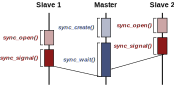
\includegraphics[width=.75\linewidth]{imgs/sync-all-to-one.pdf}
			}
			\only<2>{
				\begin{itemize}
					\item Provides cluster synchronization across \textbf{distributed barriers}
					\item Analogous to POSIX Signals
					\item Two modes
					\begin{itemize}
						\item \texttt{ALL\_TO\_ONE}
						\item \textbf{\texttt{ONE\_TO\_ALL}}
					\end{itemize}
				\end{itemize}
				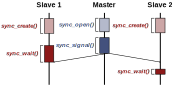
\includegraphics[width=.75\linewidth]{imgs/sync-one-to-all.pdf}
			}
		\end{overprint}

			% \textit{Synchronization Abstraction}, called \sync, provides the
			% basis for cluster synchronization across distributed barriers.
			% Its behavior is analogous to \posix Signals abstraction, but
			% notifications do not carry information, they are only for synchronization.
			% \sync defines two synchronization modes, \texttt{ALL\_TO\_ONE} and
			% \texttt{ONE\_TO\_ALL}. In both modes, there is a single master node
			% (\texttt{ONE}) and one or more slave nodes
			% (\texttt{ALL}) involved in the communication. \autoref{fig:sync-all-to-one} illustrates the
			% \texttt{ALL\_TO\_ONE} mode, where the master node waits blocked for
			% the $N$ notifications coming from the slaves. In contrast,
			% \autoref{fig:sync-one-to-all} pictures the \texttt{ONE\_TO\_ALL} mode,
			% where the master notifies the $N$ slaves, releasing them from the lock.
			% The sender nodes are responsible for sending a signal and will never
			% block. Receiver nodes are responsible for waiting for all notifications
			% to arrive.
		\end{frame}

		% \pholder[Implementation]{Sync Abstration Implementation}
		\begin{frame}[fragile]{Sync Abstration Implementation}
			\begin{itemize}
				\item Parameters required
				\begin{itemize}
					\item Node list
					\item List size
					\item Mode
				\end{itemize}
				\item Master node must be the first on the list
			\end{itemize}

			\begin{itemize}
				\item Resources required
				\begin{itemize}
					\item Create: 1 RX CNoC
					\item Open: 1 TX CNoC
				\end{itemize}
			\end{itemize}

			\begin{itemize}
				\item Simultaneous operations
				\begin{itemize}
					\item Create: 24
					\item Open: 1
				\end{itemize}
			\end{itemize}
		\end{frame}

		% \pholder[Concept]{Mailbox Abstration Concept}
		\begin{frame}[fragile]{Mailbox Abstration}
			\begin{itemize}
				\item Allows exchange fixed-length message
				\item Similarly to POSIX Message Queue
				\item Receiver allocates space to N messages
				\item Sender transfer to predefined location
			\end{itemize}

			\addfig[][width=.5\linewidth]{mailbox-concept.pdf}
			\addfig[][width=.5\linewidth]{mailbox-flow.pdf}			

			% \textit{Message Queue Abstraction}, called \mailbox, allows clusters to exchange
			% fixed-length messages with each other. The message size is designed to be
			% relatively small, usually a few hundreds of bytes. The recipient consumes these
			% messages without needing to know who sent them. Similarly, mailbox operations
			% follow the behavior of the \posix message queue. \autoref{fig:mailbox-concept}
			% conceptually illustrates one of the ways to implement a \mailbox. The receiver
			% allocates enough space to receive one message from each possible sender.
			% The sender transfers the message to a predefined location.

			% \autoref{fig:mailbox-flow} outlines the communication flow between a
			% receiver and a sender node. The receiver creates an empty message queue
			% where senders are free to send the first message. Subsequently, to
			% avoid overwriting old messages, all transmissions require the permission
			% of the receiver. For this reason,  when the receiver consumes a message,
			% it copies the message to the user buffer, releases the queue space, and
			% notifies the sender.
		\end{frame}

		% \pholder[Implementation]{Mailbox Abstration Implementation}
		\begin{frame}[fragile]{Mailbox Abstration Implementation}
			\begin{itemize}
				\item Parameters required
				\begin{itemize}
					\item Node list
					\item List size
					\item Mode
				\end{itemize}
				\item Master node must be the first on the list
			\end{itemize}

			\begin{itemize}
				\item Resources required
				\begin{itemize}
					\item Create: 1 RX CNoC
					\item Open: 1 TX CNoC
				\end{itemize}
			\end{itemize}

			\begin{itemize}
				\item Simultaneous operations
				\begin{itemize}
					\item Create: 24
					\item Open: 1
				\end{itemize}
			\end{itemize}
		\end{frame}

		\pholder[Concept]{Portal Abstration Concept}

		% \pholder[Implementation]{Portal Abstration Implementation}
		\begin{frame}[fragile]{Portal Abstration Implementation}
			\begin{itemize}
				\item Parameters required
				\begin{itemize}
					\item Node list
					\item List size
					\item Mode
				\end{itemize}
				\item Master node must be the first on the list
			\end{itemize}

			\begin{itemize}
				\item Resources required
				\begin{itemize}
					\item Create: 1 RX CNoC
					\item Open: 1 TX CNoC
				\end{itemize}
			\end{itemize}

			\begin{itemize}
				\item Simultaneous operations
				\begin{itemize}
					\item Create: 24
					\item Open: 1
				\end{itemize}
			\end{itemize}
		\end{frame}

	\subsection{User-Level Communication}

		\pholder{Impacts of the Master-Slave Model}

		\pholder[Protection and Management, Multiplexing, Validation and Correctness Tests]{Details}

% LocalWords:  template cls standalone GitHub Overleaf bugfixes SVGs
% LocalWords:  Re-empacotamento fontsize Makefile pdflatex imgs PDFs
% LocalWords:  shell-escape frames SVG brazil english lapesd-slides
% LocalWords:  disabletodonotes todonotes TODO's backup showbackup
% LocalWords:  hidebackup abntexcite abntex natbib nobib titleframe
% LocalWords:  frame showsections sidebar stopcountingframes default
% LocalWords:  thanksframe Thank You Questions referencesframe titulo
% LocalWords:  bibfiles pholder todonote placeholder inline addfig
% LocalWords:  opts graphicx addfiglw width Citations dijkstra Direct
% LocalWords:  Closure Parallel dynamic scheduling DoImportantStuff
% LocalWords:  lccp merged cell svg pdf
